% Options for packages loaded elsewhere
\PassOptionsToPackage{unicode}{hyperref}
\PassOptionsToPackage{hyphens}{url}
%
\documentclass[
]{book}
\usepackage{amsmath,amssymb}
\usepackage{iftex}
\ifPDFTeX
  \usepackage[T1]{fontenc}
  \usepackage[utf8]{inputenc}
  \usepackage{textcomp} % provide euro and other symbols
\else % if luatex or xetex
  \usepackage{unicode-math} % this also loads fontspec
  \defaultfontfeatures{Scale=MatchLowercase}
  \defaultfontfeatures[\rmfamily]{Ligatures=TeX,Scale=1}
\fi
\usepackage{lmodern}
\ifPDFTeX\else
  % xetex/luatex font selection
\fi
% Use upquote if available, for straight quotes in verbatim environments
\IfFileExists{upquote.sty}{\usepackage{upquote}}{}
\IfFileExists{microtype.sty}{% use microtype if available
  \usepackage[]{microtype}
  \UseMicrotypeSet[protrusion]{basicmath} % disable protrusion for tt fonts
}{}
\makeatletter
\@ifundefined{KOMAClassName}{% if non-KOMA class
  \IfFileExists{parskip.sty}{%
    \usepackage{parskip}
  }{% else
    \setlength{\parindent}{0pt}
    \setlength{\parskip}{6pt plus 2pt minus 1pt}}
}{% if KOMA class
  \KOMAoptions{parskip=half}}
\makeatother
\usepackage{xcolor}
\usepackage{color}
\usepackage{fancyvrb}
\newcommand{\VerbBar}{|}
\newcommand{\VERB}{\Verb[commandchars=\\\{\}]}
\DefineVerbatimEnvironment{Highlighting}{Verbatim}{commandchars=\\\{\}}
% Add ',fontsize=\small' for more characters per line
\usepackage{framed}
\definecolor{shadecolor}{RGB}{248,248,248}
\newenvironment{Shaded}{\begin{snugshade}}{\end{snugshade}}
\newcommand{\AlertTok}[1]{\textcolor[rgb]{0.94,0.16,0.16}{#1}}
\newcommand{\AnnotationTok}[1]{\textcolor[rgb]{0.56,0.35,0.01}{\textbf{\textit{#1}}}}
\newcommand{\AttributeTok}[1]{\textcolor[rgb]{0.13,0.29,0.53}{#1}}
\newcommand{\BaseNTok}[1]{\textcolor[rgb]{0.00,0.00,0.81}{#1}}
\newcommand{\BuiltInTok}[1]{#1}
\newcommand{\CharTok}[1]{\textcolor[rgb]{0.31,0.60,0.02}{#1}}
\newcommand{\CommentTok}[1]{\textcolor[rgb]{0.56,0.35,0.01}{\textit{#1}}}
\newcommand{\CommentVarTok}[1]{\textcolor[rgb]{0.56,0.35,0.01}{\textbf{\textit{#1}}}}
\newcommand{\ConstantTok}[1]{\textcolor[rgb]{0.56,0.35,0.01}{#1}}
\newcommand{\ControlFlowTok}[1]{\textcolor[rgb]{0.13,0.29,0.53}{\textbf{#1}}}
\newcommand{\DataTypeTok}[1]{\textcolor[rgb]{0.13,0.29,0.53}{#1}}
\newcommand{\DecValTok}[1]{\textcolor[rgb]{0.00,0.00,0.81}{#1}}
\newcommand{\DocumentationTok}[1]{\textcolor[rgb]{0.56,0.35,0.01}{\textbf{\textit{#1}}}}
\newcommand{\ErrorTok}[1]{\textcolor[rgb]{0.64,0.00,0.00}{\textbf{#1}}}
\newcommand{\ExtensionTok}[1]{#1}
\newcommand{\FloatTok}[1]{\textcolor[rgb]{0.00,0.00,0.81}{#1}}
\newcommand{\FunctionTok}[1]{\textcolor[rgb]{0.13,0.29,0.53}{\textbf{#1}}}
\newcommand{\ImportTok}[1]{#1}
\newcommand{\InformationTok}[1]{\textcolor[rgb]{0.56,0.35,0.01}{\textbf{\textit{#1}}}}
\newcommand{\KeywordTok}[1]{\textcolor[rgb]{0.13,0.29,0.53}{\textbf{#1}}}
\newcommand{\NormalTok}[1]{#1}
\newcommand{\OperatorTok}[1]{\textcolor[rgb]{0.81,0.36,0.00}{\textbf{#1}}}
\newcommand{\OtherTok}[1]{\textcolor[rgb]{0.56,0.35,0.01}{#1}}
\newcommand{\PreprocessorTok}[1]{\textcolor[rgb]{0.56,0.35,0.01}{\textit{#1}}}
\newcommand{\RegionMarkerTok}[1]{#1}
\newcommand{\SpecialCharTok}[1]{\textcolor[rgb]{0.81,0.36,0.00}{\textbf{#1}}}
\newcommand{\SpecialStringTok}[1]{\textcolor[rgb]{0.31,0.60,0.02}{#1}}
\newcommand{\StringTok}[1]{\textcolor[rgb]{0.31,0.60,0.02}{#1}}
\newcommand{\VariableTok}[1]{\textcolor[rgb]{0.00,0.00,0.00}{#1}}
\newcommand{\VerbatimStringTok}[1]{\textcolor[rgb]{0.31,0.60,0.02}{#1}}
\newcommand{\WarningTok}[1]{\textcolor[rgb]{0.56,0.35,0.01}{\textbf{\textit{#1}}}}
\usepackage{longtable,booktabs,array}
\usepackage{calc} % for calculating minipage widths
% Correct order of tables after \paragraph or \subparagraph
\usepackage{etoolbox}
\makeatletter
\patchcmd\longtable{\par}{\if@noskipsec\mbox{}\fi\par}{}{}
\makeatother
% Allow footnotes in longtable head/foot
\IfFileExists{footnotehyper.sty}{\usepackage{footnotehyper}}{\usepackage{footnote}}
\makesavenoteenv{longtable}
\usepackage{graphicx}
\makeatletter
\def\maxwidth{\ifdim\Gin@nat@width>\linewidth\linewidth\else\Gin@nat@width\fi}
\def\maxheight{\ifdim\Gin@nat@height>\textheight\textheight\else\Gin@nat@height\fi}
\makeatother
% Scale images if necessary, so that they will not overflow the page
% margins by default, and it is still possible to overwrite the defaults
% using explicit options in \includegraphics[width, height, ...]{}
\setkeys{Gin}{width=\maxwidth,height=\maxheight,keepaspectratio}
% Set default figure placement to htbp
\makeatletter
\def\fps@figure{htbp}
\makeatother
\setlength{\emergencystretch}{3em} % prevent overfull lines
\providecommand{\tightlist}{%
  \setlength{\itemsep}{0pt}\setlength{\parskip}{0pt}}
\setcounter{secnumdepth}{5}
\usepackage{booktabs}
\usepackage{listings}
\lstset{breaklines=true}
\ifLuaTeX
  \usepackage{selnolig}  % disable illegal ligatures
\fi
\usepackage[]{natbib}
\bibliographystyle{plainnat}
\usepackage{bookmark}
\IfFileExists{xurl.sty}{\usepackage{xurl}}{} % add URL line breaks if available
\urlstyle{same}
\hypersetup{
  pdftitle={GAM-NICHE: Shape-Constrained GAMs to build Species Distribution Models under the ecological niche theory},
  pdfauthor={AZTI},
  hidelinks,
  pdfcreator={LaTeX via pandoc}}

\title{GAM-NICHE: Shape-Constrained GAMs to build Species Distribution Models under the ecological niche theory}
\author{AZTI}
\date{2025-02-14}

\begin{document}
\maketitle

{
\setcounter{tocdepth}{1}
\tableofcontents
}
\chapter*{About}\label{about}
\addcontentsline{toc}{chapter}{About}

This is a short tutorial for constructing Species Distribution Models in R using Shape-Constrained Generalized Additive Models \citep{pya_etal_2015}, based on the development and application to marine fish by \citet{citores_etal_2020}.

The code is available in \href{https://github.com/Fundacion-AZTI/gam-niche}{AZTI's github repository} and the book is readily available \href{https://fundacion-azti.github.io/gam-niche/}{here}.This work is licensed under a \href{https://creativecommons.org/licenses/by-nc-sa/4.0/}{Creative Commons Attribution-NonCommercial-ShareAlike 4.0 International License (CC BY-NC-SA 4.0)}

To cite this book, please use:

Valle, M., Citores, L., Ibaibarriaga, L., Chust, C. (2023) GAM-NICHE: Shape-Constrained GAMs to build Species Distribution Models under the ecological niche theory. AZTI. \url{https://doi.org/10.57762/fzpy-6w51}

\chapter{Introduction}\label{introduction}

Species Distribution Models (SDMs) are numerical tools that combine observations of species occurrence or abundance at known locations with information on the environmental and/or spatial characteristics of those locations \citep{elith_etal_2009}. SDMs are widely used as a tool for understanding species spatial ecology and are also known as ecological niche models (ENM) or habitat suitability models.

According to ecological niche theory, species response curves are unimodal with respect to environmental gradients \citep{hutchinson_1957}. While a variety of statistical methods have been developed for species distribution modelling, a general problem with most of these habitat modelling approaches is that the estimated response curves can display biologically implausible shapes which do not respect ecological niche theory. This is because species response curves are fit statistically with any assumption or restriction, which sometimes do not respect the ecological niche theory. To better understand species response to environmental changes, SDMs should consider theoretical background such as the ecological niche theory and pursue the unimodality of the response curves with respect to environmental gradients.

This book provides a tutorial on how to use Shape-Constrained Generalized Additive Models (SC-GAMs) \citep{pya_etal_2015} to build SDMs under the ecological niche theory framework \citep{citores_etal_2020}. SC-GAMs impose monotonicity and concavity constraints in the linear predictor of the GAMs and avoid overfitting. SC-GAM is an effective alternative to fitting nonsymmetric parametric response curves, while retaining the unimodality constraint, required by ecological niche theory, for direct variables and limiting factors.

The book is organised following the key steps in good modelling practice of SDMs \citep{elith_etal_2009}. First, presence data of a selected species are downloaded from GBIF/OBIS global public datasets and pseudo-absence data are created. Then, environmental data are downloaded from public repositories and extracted at each of the presence/pseudo-absence data points. Based on this dataset, an exploratory analysis is conducted to help deciding on the best modelling approach. The model is fitted to the dataset and the quality of the fit and the realism of the fitted response function are evaluated. After selecting a threshold to transform the continuous probability predictions into binary responses, the model is validated using a k-fold approach. Finally, the predicted maps are generated for visualization.

\chapter{Presence-absence data}\label{presence-absence-data}

In this chapter we first, download occurrence data from global open-access datasets such as Global Biodiversity Information Facility (GBIF, \url{https://www.gbif.org/}) and Ocean Biodiversity Information System (OBIS, \url{https://obis.org/}); second, clean downloaded data reformating, renaming fields and removing outliers data; and lastly, we generate a set of pseudoabsence points along the defined study area.

First we load a list of required libraries.

\begin{Shaded}
\begin{Highlighting}[]
\NormalTok{requiredPackages }\OtherTok{\textless{}{-}} \FunctionTok{c}\NormalTok{(}\StringTok{"here"}\NormalTok{, }\StringTok{"rstudioapi"}\NormalTok{,}
    \StringTok{"ggplot2"}\NormalTok{, }\StringTok{"robis"}\NormalTok{, }\StringTok{"rgbif"}\NormalTok{, }\StringTok{"CoordinateCleaner"}\NormalTok{,}
    \StringTok{"sf"}\NormalTok{, }\StringTok{"data.table"}\NormalTok{, }\StringTok{"dplyr"}\NormalTok{, }\StringTok{"tidyr"}\NormalTok{,}
    \StringTok{"marmap"}\NormalTok{, }\StringTok{"tidyverse"}\NormalTok{, }\StringTok{"scales"}\NormalTok{, }\StringTok{"ggridges"}\NormalTok{,}
    \StringTok{"maps"}\NormalTok{, }\StringTok{"mapdata"}\NormalTok{, }\StringTok{"mapproj"}\NormalTok{, }\StringTok{"mapplots"}\NormalTok{,}
    \StringTok{"gridExtra"}\NormalTok{, }\StringTok{"lubridate"}\NormalTok{, }\StringTok{"raster"}\NormalTok{)}
\end{Highlighting}
\end{Shaded}

We run a function to install the required packages that are not in our system and load all the required packages.

\begin{Shaded}
\begin{Highlighting}[]
\NormalTok{install\_load\_function }\OtherTok{\textless{}{-}} \ControlFlowTok{function}\NormalTok{(pkg) \{}
\NormalTok{    new.pkg }\OtherTok{\textless{}{-}}\NormalTok{ pkg[}\SpecialCharTok{!}\NormalTok{(pkg }\SpecialCharTok{\%in\%} \FunctionTok{installed.packages}\NormalTok{()[,}
        \StringTok{"Package"}\NormalTok{])]}
    \ControlFlowTok{if}\NormalTok{ (}\FunctionTok{length}\NormalTok{(new.pkg))}
        \FunctionTok{install.packages}\NormalTok{(new.pkg, }\AttributeTok{dependencies =} \ConstantTok{TRUE}\NormalTok{)}
    \FunctionTok{sapply}\NormalTok{(pkg, require, }\AttributeTok{character.only =} \ConstantTok{TRUE}\NormalTok{)}
\NormalTok{\}}

\FunctionTok{install\_load\_function}\NormalTok{(requiredPackages)}
\end{Highlighting}
\end{Shaded}

\begin{verbatim}
##              here        rstudioapi           ggplot2             robis 
##              TRUE              TRUE              TRUE              TRUE 
##             rgbif CoordinateCleaner                sf        data.table 
##              TRUE              TRUE              TRUE              TRUE 
##             dplyr             tidyr            marmap         tidyverse 
##              TRUE              TRUE              TRUE              TRUE 
##            scales          ggridges              maps           mapdata 
##              TRUE              TRUE              TRUE              TRUE 
##           mapproj          mapplots         gridExtra         lubridate 
##              TRUE              TRUE              TRUE              TRUE 
##            raster 
##              TRUE
\end{verbatim}

We define some overall settings.

\begin{Shaded}
\begin{Highlighting}[]
\CommentTok{\# General settings for ggplot}
\CommentTok{\# (black{-}white background, larger}
\CommentTok{\# base\_size)}
\FunctionTok{theme\_set}\NormalTok{(}\FunctionTok{theme\_bw}\NormalTok{(}\AttributeTok{base\_size =} \DecValTok{16}\NormalTok{))}
\end{Highlighting}
\end{Shaded}

\section{Download presence data}\label{download-presence-data}

In this section we download presence data from global public datasets.

To do so, we first define a study area, in this case we select the Atlantic Ocean based on the The Food and Agriculture Organization (FAO) Major Fishing Areas for Statistical Purposes and we remove Black Sea subarea.

\begin{Shaded}
\begin{Highlighting}[]
\CommentTok{\# we could download the shapefile with}
\CommentTok{\# the FAO fishing areas from the url}
\CommentTok{\# where FAO shapefile is stored}
\CommentTok{\# uncommenting the next two lines:}

\CommentTok{\# url\textless{}{-}\textquotesingle{}https://www.fao.org/fishery/geoserver/area/ows?service=WFS\&version=1.0.0\&request=GetFeature\&typeName=area\%3AFAO\_AREAS\&maxFeatures=50\&outputFormat=SHAPE{-}ZIP\textquotesingle{}}
\CommentTok{\# download.file(url,\textquotesingle{}data/spatial/FAO\_AREAS.zip\textquotesingle{},mode=\textquotesingle{}wb\textquotesingle{})}

\CommentTok{\# Unzip downloaded file}
\FunctionTok{unzip}\NormalTok{(here}\SpecialCharTok{::}\FunctionTok{here}\NormalTok{(}\StringTok{"data"}\NormalTok{, }\StringTok{"spatial"}\NormalTok{, }\StringTok{"FAO\_AREAS.zip"}\NormalTok{),}
    \AttributeTok{exdir =} \StringTok{"data/spatial"}\NormalTok{)}

\CommentTok{\# Load FAO (spatial multipolygon)}
\NormalTok{FAO }\OtherTok{\textless{}{-}} \FunctionTok{st\_read}\NormalTok{(}\FunctionTok{file.path}\NormalTok{(}\StringTok{"data"}\NormalTok{, }\StringTok{"spatial"}\NormalTok{,}
    \StringTok{"FAO\_AREAS.shp"}\NormalTok{))}
\end{Highlighting}
\end{Shaded}

\begin{verbatim}
## Reading layer `FAO_AREAS' from data source 
##   `C:\USE\GitHub\gam-niche\data\spatial\FAO_AREAS.shp' using driver `ESRI Shapefile'
## Simple feature collection with 50 features and 15 fields
## Geometry type: MULTIPOLYGON
## Dimension:     XY
## Bounding box:  xmin: -180 ymin: -85.58276 xmax: 180 ymax: 89.99
## Geodetic CRS:  WGS 84
\end{verbatim}

\begin{Shaded}
\begin{Highlighting}[]
\CommentTok{\# Select Atlantic Ocean FAO Area}
\NormalTok{FAO\_Atl }\OtherTok{\textless{}{-}}\NormalTok{ FAO[FAO}\SpecialCharTok{$}\NormalTok{OCEAN }\SpecialCharTok{==} \StringTok{"Atlantic"}\NormalTok{, ]}

\CommentTok{\# Select Black Sea subarea}
\NormalTok{Black\_Sea }\OtherTok{\textless{}{-}}\NormalTok{ FAO\_Atl[FAO\_Atl}\SpecialCharTok{$}\NormalTok{ID }\SpecialCharTok{==} \StringTok{"20"}\NormalTok{,}
\NormalTok{    ]}

\CommentTok{\# Transform to sf objects}
\NormalTok{FAO\_Atl.sf }\OtherTok{\textless{}{-}} \FunctionTok{st\_as\_sf}\NormalTok{(FAO\_Atl)}
\NormalTok{Black\_Sea.sf }\OtherTok{\textless{}{-}} \FunctionTok{st\_as\_sf}\NormalTok{(Black\_Sea)}

\CommentTok{\# Remove Black sea using st\_difference}
\CommentTok{\# (reverse of st\_intersection)}
\NormalTok{FAO\_Atl\_no\_black\_sea }\OtherTok{\textless{}{-}} \FunctionTok{st\_difference}\NormalTok{(FAO\_Atl.sf,}
\NormalTok{    Black\_Sea.sf) }\SpecialCharTok{\%\textgreater{}\%}
\NormalTok{    dplyr}\SpecialCharTok{::}\FunctionTok{select}\NormalTok{(F\_AREA)}

\CommentTok{\# Transform to spatial polygons}
\CommentTok{\# dataframe}
\NormalTok{study\_area }\OtherTok{\textless{}{-}}\NormalTok{ sf}\SpecialCharTok{:::}\FunctionTok{as\_Spatial}\NormalTok{(FAO\_Atl\_no\_black\_sea)}

\FunctionTok{plot}\NormalTok{(study\_area)}
\end{Highlighting}
\end{Shaded}

\includegraphics{_main_files/figure-latex/unnamed-chunk-6-1.pdf}

\begin{Shaded}
\begin{Highlighting}[]
\CommentTok{\# Remove unused files}
\FunctionTok{rm}\NormalTok{(FAO, FAO\_Atl, FAO\_Atl.sf, FAO\_Atl\_no\_black\_sea,}
\NormalTok{    Black\_Sea, Black\_Sea.sf)}
\end{Highlighting}
\end{Shaded}

Download occurrence data from OBIS and GBIF using scientific name.

In this case we select Albacore tuna species (Thunnus alalunga). This can take a long time, so we upload data downloaded previously.

\begin{Shaded}
\begin{Highlighting}[]
\CommentTok{\# To get data from OBIS}
\CommentTok{\# mydata.obis\textless{}{-}robis::occurrence(scientificname=\textquotesingle{}Thunnus}
\CommentTok{\# alalunga\textquotesingle{})}

\CommentTok{\# To get data from GBIF}
\CommentTok{\# mydata.gbif\textless{}{-}occ\_data(scientificName=\textquotesingle{}Thunnus}
\CommentTok{\# alalunga\textquotesingle{}, hasCoordinate = TRUE,}
\CommentTok{\# limit=100000)$data}

\CommentTok{\# Given that this can take a long time,}
\CommentTok{\# we upload data downloaded previously}
\FunctionTok{load}\NormalTok{(here}\SpecialCharTok{::}\FunctionTok{here}\NormalTok{(}\StringTok{"data"}\NormalTok{, }\StringTok{"occurrences"}\NormalTok{, }\StringTok{"mydata.obis.RData"}\NormalTok{))}
\FunctionTok{load}\NormalTok{(here}\SpecialCharTok{::}\FunctionTok{here}\NormalTok{(}\StringTok{"data"}\NormalTok{, }\StringTok{"occurrences"}\NormalTok{, }\StringTok{"mydata.gbif.RData"}\NormalTok{))}
\end{Highlighting}
\end{Shaded}

We now check the downloaded data and select the fields of interest.

\begin{Shaded}
\begin{Highlighting}[]
\CommentTok{\# Check names for GBIF data}
\FunctionTok{names}\NormalTok{(mydata.gbif)}
\end{Highlighting}
\end{Shaded}

\begin{verbatim}
##   [1] "key"                              "scientificName"                  
##   [3] "decimalLatitude"                  "decimalLongitude"                
##   [5] "issues"                           "datasetKey"                      
##   [7] "publishingOrgKey"                 "installationKey"                 
##   [9] "publishingCountry"                "protocol"                        
##  [11] "lastCrawled"                      "lastParsed"                      
##  [13] "crawlId"                          "hostingOrganizationKey"          
##  [15] "basisOfRecord"                    "occurrenceStatus"                
##  [17] "taxonKey"                         "kingdomKey"                      
##  [19] "phylumKey"                        "orderKey"                        
##  [21] "familyKey"                        "genusKey"                        
##  [23] "speciesKey"                       "acceptedTaxonKey"                
##  [25] "acceptedScientificName"           "kingdom"                         
##  [27] "phylum"                           "order"                           
##  [29] "family"                           "genus"                           
##  [31] "species"                          "genericName"                     
##  [33] "specificEpithet"                  "taxonRank"                       
##  [35] "taxonomicStatus"                  "iucnRedListCategory"             
##  [37] "dateIdentified"                   "coordinateUncertaintyInMeters"   
##  [39] "year"                             "month"                           
##  [41] "day"                              "eventDate"                       
##  [43] "modified"                         "lastInterpreted"                 
##  [45] "references"                       "license"                         
##  [47] "isInCluster"                      "datasetName"                     
##  [49] "recordedBy"                       "identifiedBy"                    
##  [51] "geodeticDatum"                    "countryCode"                     
##  [53] "country"                          "rightsHolder"                    
##  [55] "identifier"                       "http://unknown.org/nick"         
##  [57] "informationWithheld"              "verbatimEventDate"               
##  [59] "collectionCode"                   "gbifID"                          
##  [61] "occurrenceID"                     "taxonID"                         
##  [63] "catalogNumber"                    "institutionCode"                 
##  [65] "eventTime"                        "http://unknown.org/captive"      
##  [67] "identificationID"                 "continent"                       
##  [69] "stateProvince"                    "verbatimLocality"                
##  [71] "occurrenceRemarks"                "lifeStage"                       
##  [73] "datasetID"                        "eventID"                         
##  [75] "footprintWKT"                     "originalNameUsage"               
##  [77] "county"                           "identificationVerificationStatus"
##  [79] "nameAccordingTo"                  "networkKeys"                     
##  [81] "individualCount"                  "elevation"                       
##  [83] "waterBody"                        "institutionKey"                  
##  [85] "otherCatalogNumbers"              "preparations"                    
##  [87] "recordNumber"                     "acceptedNameUsage"               
##  [89] "vernacularName"                   "institutionID"                   
##  [91] "language"                         "type"                            
##  [93] "identificationRemarks"            "projectId"                       
##  [95] "municipality"                     "collectionKey"                   
##  [97] "higherGeography"                  "georeferenceProtocol"            
##  [99] "island"                           "endDayOfYear"                    
## [101] "locality"                         "fieldNumber"                     
## [103] "startDayOfYear"                   "collectionID"                    
## [105] "higherClassification"             "materialSampleID"                
## [107] "disposition"                      "programmeAcronym"                
## [109] "organismQuantity"                 "organismQuantityType"            
## [111] "samplingProtocol"                 "locationAccordingTo"             
## [113] "coordinatePrecision"              "georeferencedDate"               
## [115] "nomenclaturalCode"                "associatedReferences"            
## [117] "taxonRemarks"                     "ownerInstitutionCode"            
## [119] "bibliographicCitation"            "habitat"                         
## [121] "locationRemarks"                  "depth"                           
## [123] "http://unknown.org/license"       "taxonConceptID"                  
## [125] "http://unknown.org/rightsHolder"  "depthAccuracy"                   
## [127] "dynamicProperties"                "elevationAccuracy"               
## [129] "rights"                           "georeferenceSources"             
## [131] "georeferenceRemarks"              "name"                            
## [133] "associatedSequences"              "establishmentMeans"              
## [135] "georeferenceVerificationStatus"   "accessRights"                    
## [137] "georeferencedBy"                  "verbatimSRS"                     
## [139] "previousIdentifications"          "locationID"                      
## [141] "acceptedNameUsageID"              "http://unknown.org/language"     
## [143] "http://unknown.org/modified"      "samplingEffort"                  
## [145] "verbatimDepth"                    "behavior"                        
## [147] "eventRemarks"                     "footprintSRS"                    
## [149] "namePublishedInYear"              "verbatimCoordinateSystem"        
## [151] "parentNameUsage"                  "http://unknown.org/taxonRankID"  
## [153] "http://unknown.org/species"       "higherGeographyID"               
## [155] "islandGroup"                      "organismID"                      
## [157] "distanceFromCentroidInMeters"     "http://unknown.org/orders"       
## [159] "typeStatus"
\end{verbatim}

\begin{Shaded}
\begin{Highlighting}[]
\CommentTok{\# Select columns of interest}
\NormalTok{mydata.gbif }\OtherTok{\textless{}{-}}\NormalTok{ mydata.gbif }\SpecialCharTok{\%\textgreater{}\%}
\NormalTok{    dplyr}\SpecialCharTok{::}\FunctionTok{select}\NormalTok{(}\StringTok{"acceptedScientificName"}\NormalTok{,}
        \StringTok{"decimalLongitude"}\NormalTok{, }\StringTok{"decimalLatitude"}\NormalTok{,}
        \StringTok{"year"}\NormalTok{, }\StringTok{"month"}\NormalTok{, }\StringTok{"day"}\NormalTok{, }\StringTok{"eventDate"}\NormalTok{,}
        \StringTok{"depth"}\NormalTok{)}

\CommentTok{\# Check names in for OBIS data}
\FunctionTok{names}\NormalTok{(mydata.obis)}
\end{Highlighting}
\end{Shaded}

\begin{verbatim}
##   [1] "infraphylum"                    "country"                       
##   [3] "date_year"                      "scientificNameID"              
##   [5] "year"                           "scientificName"                
##   [7] "dropped"                        "gigaclassid"                   
##   [9] "aphiaID"                        "decimalLatitude"               
##  [11] "subclassid"                     "gigaclass"                     
##  [13] "infraphylumid"                  "phylumid"                      
##  [15] "familyid"                       "catalogNumber"                 
##  [17] "basisOfRecord"                  "terrestrial"                   
##  [19] "id"                             "day"                           
##  [21] "parvphylum"                     "order"                         
##  [23] "dataset_id"                     "locality"                      
##  [25] "decimalLongitude"               "collectionCode"                
##  [27] "date_end"                       "speciesid"                     
##  [29] "date_start"                     "month"                         
##  [31] "genus"                          "eventDate"                     
##  [33] "brackish"                       "absence"                       
##  [35] "subfamily"                      "genusid"                       
##  [37] "originalScientificName"         "marine"                        
##  [39] "subphylumid"                    "subfamilyid"                   
##  [41] "institutionCode"                "date_mid"                      
##  [43] "class"                          "orderid"                       
##  [45] "waterBody"                      "kingdom"                       
##  [47] "classid"                        "phylum"                        
##  [49] "species"                        "subphylum"                     
##  [51] "subclass"                       "family"                        
##  [53] "category"                       "kingdomid"                     
##  [55] "parvphylumid"                   "node_id"                       
##  [57] "flags"                          "sss"                           
##  [59] "shoredistance"                  "sst"                           
##  [61] "bathymetry"                     "maximumDepthInMeters"          
##  [63] "minimumDepthInMeters"           "sex"                           
##  [65] "depth"                          "coordinatePrecision"           
##  [67] "verbatimCoordinates"            "occurrenceRemarks"             
##  [69] "individualCount"                "occurrenceStatus"              
##  [71] "modified"                       "materialSampleID"              
##  [73] "occurrenceID"                   "scientificNameAuthorship"      
##  [75] "taxonRank"                      "datasetID"                     
##  [77] "associatedReferences"           "bibliographicCitation"         
##  [79] "coordinateUncertaintyInMeters"  "vernacularName"                
##  [81] "footprintWKT"                   "specificEpithet"               
##  [83] "recordNumber"                   "georeferenceRemarks"           
##  [85] "stateProvince"                  "continent"                     
##  [87] "recordedBy"                     "rightsHolder"                  
##  [89] "language"                       "type"                          
##  [91] "license"                        "ownerInstitutionCode"          
##  [93] "datasetName"                    "geodeticDatum"                 
##  [95] "accessRights"                   "dynamicProperties"             
##  [97] "county"                         "samplingEffort"                
##  [99] "lifeStage"                      "footprintSRS"                  
## [101] "samplingProtocol"               "parentEventID"                 
## [103] "eventID"                        "eventRemarks"                  
## [105] "identifiedBy"                   "georeferencedBy"               
## [107] "minimumElevationInMeters"       "maximumElevationInMeters"      
## [109] "dateIdentified"                 "behavior"                      
## [111] "georeferenceProtocol"           "verbatimDepth"                 
## [113] "organismQuantity"               "organismQuantityType"          
## [115] "startDayOfYear"                 "collectionID"                  
## [117] "typeStatus"                     "institutionID"                 
## [119] "acceptedNameUsage"              "preparations"                  
## [121] "countryCode"                    "otherCatalogNumbers"           
## [123] "references"                     "fieldNumber"                   
## [125] "endDayOfYear"                   "eventTime"                     
## [127] "locationID"                     "taxonRemarks"                  
## [129] "georeferencedDate"              "verbatimEventDate"             
## [131] "identificationRemarks"          "nomenclaturalCode"             
## [133] "taxonomicStatus"                "higherClassification"          
## [135] "higherGeography"                "verbatimLatitude"              
## [137] "verbatimLongitude"              "establishmentMeans"            
## [139] "verbatimLocality"               "georeferenceVerificationStatus"
## [141] "island"                         "identificationQualifier"       
## [143] "identificationID"               "informationWithheld"           
## [145] "islandGroup"                    "acceptedNameUsageID"           
## [147] "locationRemarks"                "verbatimSRS"                   
## [149] "previousIdentifications"
\end{verbatim}

\begin{Shaded}
\begin{Highlighting}[]
\CommentTok{\# Select columns of interest}
\NormalTok{mydata.obis }\OtherTok{\textless{}{-}}\NormalTok{ mydata.obis }\SpecialCharTok{\%\textgreater{}\%}
\NormalTok{    dplyr}\SpecialCharTok{::}\FunctionTok{select}\NormalTok{(}\StringTok{"scientificName"}\NormalTok{, }\StringTok{"decimalLongitude"}\NormalTok{,}
        \StringTok{"decimalLatitude"}\NormalTok{, }\StringTok{"date\_year"}\NormalTok{, }\StringTok{"month"}\NormalTok{,}
        \StringTok{"day"}\NormalTok{, }\StringTok{"eventDate"}\NormalTok{, }\StringTok{"depth"}\NormalTok{, }\StringTok{"bathymetry"}\NormalTok{,}
        \StringTok{"occurrenceStatus"}\NormalTok{, }\StringTok{"sst"}\NormalTok{)}
\end{Highlighting}
\end{Shaded}

Reformat the data adding a new field and renaming some columns from mydata.gbif dataframe in order to have the same columns and be able to join both downloaded datasets.

\begin{Shaded}
\begin{Highlighting}[]
\NormalTok{mydata.gbif }\OtherTok{\textless{}{-}}\NormalTok{ mydata.gbif }\SpecialCharTok{\%\textgreater{}\%}
\NormalTok{    dplyr}\SpecialCharTok{::}\FunctionTok{rename}\NormalTok{(}\AttributeTok{scientificName =} \StringTok{"acceptedScientificName"}\NormalTok{) }\SpecialCharTok{\%\textgreater{}\%}
\NormalTok{    dplyr}\SpecialCharTok{::}\FunctionTok{rename}\NormalTok{(}\AttributeTok{date\_year =} \StringTok{"year"}\NormalTok{) }\SpecialCharTok{\%\textgreater{}\%}
\NormalTok{    dplyr}\SpecialCharTok{::}\FunctionTok{mutate}\NormalTok{(}\AttributeTok{bathymetry =} \ConstantTok{NA}\NormalTok{) }\SpecialCharTok{\%\textgreater{}\%}
\NormalTok{    dplyr}\SpecialCharTok{::}\FunctionTok{mutate}\NormalTok{(}\AttributeTok{occurrenceStatus =} \DecValTok{1}\NormalTok{) }\SpecialCharTok{\%\textgreater{}\%}
\NormalTok{    dplyr}\SpecialCharTok{::}\FunctionTok{mutate}\NormalTok{(}\AttributeTok{sst =} \ConstantTok{NA}\NormalTok{)}

\CommentTok{\# Join data from OBIS and GBIF}
\NormalTok{mydata.fus }\OtherTok{\textless{}{-}} \FunctionTok{rbind}\NormalTok{(mydata.obis, mydata.gbif)}

\CommentTok{\# Assign unique scientific name}
\NormalTok{mydata.fus }\OtherTok{\textless{}{-}}\NormalTok{ mydata.fus }\SpecialCharTok{\%\textgreater{}\%}
\NormalTok{    dplyr}\SpecialCharTok{::}\FunctionTok{mutate}\NormalTok{(}\AttributeTok{scientificName =} \FunctionTok{paste}\NormalTok{(mydata.obis}\SpecialCharTok{$}\NormalTok{scientificName[}\DecValTok{1}\NormalTok{]))}

\CommentTok{\# Remove unused files}
\FunctionTok{rm}\NormalTok{(mydata.gbif, mydata.obis)}
\end{Highlighting}
\end{Shaded}

We now clean downloaded raw data.

\begin{Shaded}
\begin{Highlighting}[]
\CommentTok{\# Give date format to eventDate and}
\CommentTok{\# fill out month and date\_year columns}
\NormalTok{mydata.fus}\SpecialCharTok{$}\NormalTok{eventDate }\OtherTok{\textless{}{-}} \FunctionTok{as.Date}\NormalTok{(mydata.fus}\SpecialCharTok{$}\NormalTok{eventDate)}
\NormalTok{mydata.fus}\SpecialCharTok{$}\NormalTok{date\_year }\OtherTok{\textless{}{-}} \FunctionTok{as.numeric}\NormalTok{(mydata.fus}\SpecialCharTok{$}\NormalTok{date\_year)}
\NormalTok{mydata.fus}\SpecialCharTok{$}\NormalTok{month }\OtherTok{\textless{}{-}} \FunctionTok{as.numeric}\NormalTok{(mydata.fus}\SpecialCharTok{$}\NormalTok{month)}

\CommentTok{\# Assign 1 value to occurrenceStatus}
\NormalTok{mydata.fus }\OtherTok{\textless{}{-}}\NormalTok{ mydata.fus }\SpecialCharTok{\%\textgreater{}\%}
\NormalTok{    dplyr}\SpecialCharTok{::}\FunctionTok{mutate}\NormalTok{(}\AttributeTok{occurrenceStatus =} \DecValTok{1}\NormalTok{)}
\end{Highlighting}
\end{Shaded}

We remove outliers based on distance method (total distance= 1000 km) available in the \texttt{CoordinateCleaner} package.

\begin{Shaded}
\begin{Highlighting}[]
\NormalTok{out.dist }\OtherTok{\textless{}{-}} \FunctionTok{cc\_outl}\NormalTok{(}\AttributeTok{x =}\NormalTok{ mydata.fus, }\AttributeTok{lon =} \StringTok{"decimalLongitude"}\NormalTok{,}
    \AttributeTok{lat =} \StringTok{"decimalLatitude"}\NormalTok{, }\AttributeTok{species =} \StringTok{"scientificName"}\NormalTok{,}
    \AttributeTok{method =} \StringTok{"distance"}\NormalTok{, }\AttributeTok{tdi =} \DecValTok{1000}\NormalTok{, }\AttributeTok{thinning =}\NormalTok{ T,}
    \AttributeTok{thinning\_res =} \FloatTok{0.5}\NormalTok{, }\AttributeTok{value =} \StringTok{"flagged"}\NormalTok{)}

\CommentTok{\# Remove outliers from the data}
\NormalTok{mydata.fus }\OtherTok{\textless{}{-}}\NormalTok{ mydata.fus[out.dist, ]}
\end{Highlighting}
\end{Shaded}

Remove duplicates.

\begin{Shaded}
\begin{Highlighting}[]
\CommentTok{\# First create a vector containing}
\CommentTok{\# longitude, latitude and event date}
\CommentTok{\# information}
\NormalTok{date }\OtherTok{\textless{}{-}} \FunctionTok{cbind}\NormalTok{(mydata.fus}\SpecialCharTok{$}\NormalTok{decimalLongitude,}
\NormalTok{    mydata.fus}\SpecialCharTok{$}\NormalTok{decimalLatitude, mydata.fus}\SpecialCharTok{$}\NormalTok{eventDate)}

\CommentTok{\# Remove the duplicated records}
\NormalTok{mydata.fus }\OtherTok{\textless{}{-}}\NormalTok{ mydata.fus[}\SpecialCharTok{!}\FunctionTok{duplicated}\NormalTok{(date),}
\NormalTok{    ]}

\CommentTok{\# Remove unused files}
\FunctionTok{rm}\NormalTok{(date)}
\end{Highlighting}
\end{Shaded}

Mask retrieved occurrence data to our study area and add bathymetry value to each occurrence point.

\begin{Shaded}
\begin{Highlighting}[]
\CommentTok{\# Assign coordinate format and}
\CommentTok{\# projection to be able to use FAO}
\CommentTok{\# Atlantic as a mask}
\NormalTok{dat }\OtherTok{\textless{}{-}} \FunctionTok{data.frame}\NormalTok{(}\FunctionTok{cbind}\NormalTok{(mydata.fus}\SpecialCharTok{$}\NormalTok{decimalLongitude,}
\NormalTok{    mydata.fus}\SpecialCharTok{$}\NormalTok{decimalLatitude))}
\NormalTok{ptos }\OtherTok{\textless{}{-}} \FunctionTok{as.data.table}\NormalTok{(dat, }\AttributeTok{keep.columnnames =} \ConstantTok{TRUE}\NormalTok{)}

\FunctionTok{coordinates}\NormalTok{(ptos) }\OtherTok{\textless{}{-}} \ErrorTok{\textasciitilde{}}\NormalTok{X1 }\SpecialCharTok{+}\NormalTok{ X2}

\CommentTok{\# Assign projection}
\FunctionTok{proj4string}\NormalTok{(ptos) }\OtherTok{\textless{}{-}} \FunctionTok{proj4string}\NormalTok{(study\_area)}

\CommentTok{\# Select only occurrences from FAO}
\CommentTok{\# Atlantic}
\NormalTok{match2 }\OtherTok{\textless{}{-}} \FunctionTok{data.frame}\NormalTok{(}\FunctionTok{subset}\NormalTok{(mydata.fus, }\SpecialCharTok{!}\FunctionTok{is.na}\NormalTok{(}\FunctionTok{over}\NormalTok{(ptos,}
\NormalTok{    study\_area)[, }\DecValTok{1}\NormalTok{])))}

\CommentTok{\# Extract the FAO area of each point}
\NormalTok{match3 }\OtherTok{\textless{}{-}} \FunctionTok{data.frame}\NormalTok{(}\FunctionTok{subset}\NormalTok{(}\FunctionTok{over}\NormalTok{(ptos, study\_area),}
    \SpecialCharTok{!}\FunctionTok{is.na}\NormalTok{(}\FunctionTok{over}\NormalTok{(ptos, study\_area)[, }\DecValTok{1}\NormalTok{])))}

\CommentTok{\# Create data frame with area, name,}
\CommentTok{\# long, lat and year}
\NormalTok{df0 }\OtherTok{\textless{}{-}} \FunctionTok{cbind}\NormalTok{(}\AttributeTok{F\_AREA =}\NormalTok{ match3}\SpecialCharTok{$}\NormalTok{F\_AREA, match2)[,}
    \FunctionTok{c}\NormalTok{(}\StringTok{"F\_AREA"}\NormalTok{, }\StringTok{"scientificName"}\NormalTok{, }\StringTok{"decimalLongitude"}\NormalTok{,}
        \StringTok{"decimalLatitude"}\NormalTok{, }\StringTok{"date\_year"}\NormalTok{, }\StringTok{"occurrenceStatus"}\NormalTok{)]}

\CommentTok{\# Rename some columns}
\FunctionTok{names}\NormalTok{(df0)[}\DecValTok{3}\SpecialCharTok{:}\DecValTok{5}\NormalTok{] }\OtherTok{\textless{}{-}} \FunctionTok{c}\NormalTok{(}\StringTok{"LON"}\NormalTok{, }\StringTok{"LAT"}\NormalTok{, }\StringTok{"YEAR"}\NormalTok{)}

\FunctionTok{options}\NormalTok{(}\AttributeTok{timeout =} \DecValTok{600}\NormalTok{)}

\CommentTok{\# Add bathymetry from NOAA}
\NormalTok{bathy }\OtherTok{\textless{}{-}}\NormalTok{ marmap}\SpecialCharTok{::}\FunctionTok{getNOAA.bathy}\NormalTok{(}\AttributeTok{lon1 =} \SpecialCharTok{{-}}\DecValTok{100}\NormalTok{,}
    \AttributeTok{lon2 =} \DecValTok{30}\NormalTok{, }\AttributeTok{lat1 =} \SpecialCharTok{{-}}\DecValTok{41}\NormalTok{, }\AttributeTok{lat2 =} \DecValTok{55}\NormalTok{, }\AttributeTok{resolution =} \DecValTok{1}\NormalTok{,}
    \AttributeTok{keep =} \ConstantTok{TRUE}\NormalTok{, }\AttributeTok{antimeridian =} \ConstantTok{FALSE}\NormalTok{, }\AttributeTok{path =}\NormalTok{ here}\SpecialCharTok{::}\FunctionTok{here}\NormalTok{(}\StringTok{"data"}\NormalTok{,}
        \StringTok{"spatial"}\NormalTok{))}

\CommentTok{\# instead, we could upload a file}
\CommentTok{\# already downloaded}
\CommentTok{\# load(here::here(\textquotesingle{}data\textquotesingle{},}
\CommentTok{\# \textquotesingle{}spatial\textquotesingle{},\textquotesingle{}bathy.RData\textquotesingle{}))}

\NormalTok{df0}\SpecialCharTok{$}\NormalTok{bathymetry }\OtherTok{\textless{}{-}} \FunctionTok{get.depth}\NormalTok{(bathy, df0[,}
    \FunctionTok{c}\NormalTok{(}\StringTok{"LON"}\NormalTok{, }\StringTok{"LAT"}\NormalTok{)], }\AttributeTok{locator =}\NormalTok{ F)}\SpecialCharTok{$}\NormalTok{depth}

\CommentTok{\# Remove unused files}
\FunctionTok{rm}\NormalTok{(mydata.fus, match2, match3, dat, ptos)}
\end{Highlighting}
\end{Shaded}

We plot the occurrence data.

\begin{Shaded}
\begin{Highlighting}[]
\FunctionTok{ggplot}\NormalTok{() }\SpecialCharTok{+} \FunctionTok{geom\_path}\NormalTok{(}\AttributeTok{data =}\NormalTok{ study\_area, }\FunctionTok{aes}\NormalTok{(}\AttributeTok{x =}\NormalTok{ long,}
    \AttributeTok{y =}\NormalTok{ lat, }\AttributeTok{group =}\NormalTok{ group), }\AttributeTok{color =} \StringTok{"gray"}\NormalTok{,}
    \AttributeTok{linewidth =} \FloatTok{0.2}\NormalTok{) }\SpecialCharTok{+} \FunctionTok{geom\_point}\NormalTok{(}\AttributeTok{data =}\NormalTok{ df0,}
    \FunctionTok{aes}\NormalTok{(}\AttributeTok{x =}\NormalTok{ LON, }\AttributeTok{y =}\NormalTok{ LAT))}
\end{Highlighting}
\end{Shaded}

\includegraphics{_main_files/figure-latex/unnamed-chunk-14-1.pdf}

And, we save the data.

\begin{Shaded}
\begin{Highlighting}[]
\FunctionTok{save}\NormalTok{(df0, }\AttributeTok{file =} \StringTok{"data/occurrences/occ.RData"}\NormalTok{)}
\FunctionTok{save}\NormalTok{(study\_area, }\AttributeTok{file =} \StringTok{"data/spatial/study\_area.RData"}\NormalTok{)}
\end{Highlighting}
\end{Shaded}

\section{Create pseudo-absence data}\label{create-pseudo-absence-data}

After saving presence data for the species of interest we need to generate absence information in order to work with logistic regression SDM afterwards. In this case we create pseudo-absence data with a constant prevalence of 50\% \citep{mcpherson_2004}; \citep{barbetmassin_etal_2012}.

For that, we generate a buffer around each presence data point, with a radius of 100km, where no points can be generated.

Before starting the pseudo-absence generation process, we delete observations in land (positive bathymetry) and select data between 2000 and 2014 (same temporal range as the environmental data that we will download later).

\begin{Shaded}
\begin{Highlighting}[]
\CommentTok{\# Remove points in land}
\NormalTok{df0 }\OtherTok{\textless{}{-}} \FunctionTok{subset}\NormalTok{(df0, bathymetry }\SpecialCharTok{\textless{}} \DecValTok{0}\NormalTok{)}

\CommentTok{\# Select only years from 2000 to 2014}
\NormalTok{df0 }\OtherTok{\textless{}{-}} \FunctionTok{subset}\NormalTok{(df0, YEAR }\SpecialCharTok{\textless{}=} \DecValTok{2014} \SpecialCharTok{\&}\NormalTok{ YEAR }\SpecialCharTok{\textgreater{}=}
    \DecValTok{2000}\NormalTok{)}
\end{Highlighting}
\end{Shaded}

Then we transform the presence data frame to ``SpatialPointsDataFrame'' class object and to ``sf'' class object so we can operate and plot easily with spatial data tools. We can see the characteristics of the object through its summary.

\begin{Shaded}
\begin{Highlighting}[]
\CommentTok{\# Convert to spatial point data frame}
\NormalTok{df }\OtherTok{\textless{}{-}}\NormalTok{ df0}
\FunctionTok{coordinates}\NormalTok{(df) }\OtherTok{\textless{}{-}} \ErrorTok{\textasciitilde{}}\NormalTok{LON }\SpecialCharTok{+}\NormalTok{ LAT}
\FunctionTok{crs}\NormalTok{(df) }\OtherTok{\textless{}{-}} \FunctionTok{crs}\NormalTok{(study\_area)}

\CommentTok{\# Convert to sf}
\NormalTok{df.sf }\OtherTok{\textless{}{-}} \FunctionTok{st\_as\_sf}\NormalTok{(df)}
\NormalTok{study\_area.sf }\OtherTok{\textless{}{-}} \FunctionTok{st\_union}\NormalTok{(}\FunctionTok{st\_as\_sf}\NormalTok{(study\_area))}


\FunctionTok{summary}\NormalTok{(df)}
\end{Highlighting}
\end{Shaded}

\begin{verbatim}
## Object of class SpatialPointsDataFrame
## Coordinates:
##        min      max
## LON -95.65 24.45000
## LAT -34.71 54.15014
## Is projected: FALSE 
## proj4string : [+proj=longlat +datum=WGS84 +no_defs]
## Number of points: 14903
## Data attributes:
##     F_AREA          scientificName          YEAR      occurrenceStatus
##  Length:14903       Length:14903       Min.   :2000   Min.   :1       
##  Class :character   Class :character   1st Qu.:2001   1st Qu.:1       
##  Mode  :character   Mode  :character   Median :2002   Median :1       
##                                        Mean   :2003   Mean   :1       
##                                        3rd Qu.:2004   3rd Qu.:1       
##                                        Max.   :2013   Max.   :1       
##    bathymetry      
##  Min.   :-8404.09  
##  1st Qu.:-1916.92  
##  Median :-1030.77  
##  Mean   :-1433.61  
##  3rd Qu.: -351.32  
##  Max.   :   -1.13
\end{verbatim}

We can easily plot sf objects using ggplot, here we plot the area of study and the presence data points.

\begin{Shaded}
\begin{Highlighting}[]
\FunctionTok{ggplot}\NormalTok{(study\_area.sf) }\SpecialCharTok{+} \FunctionTok{geom\_sf}\NormalTok{() }\SpecialCharTok{+} \FunctionTok{geom\_sf}\NormalTok{(}\AttributeTok{data =} \FunctionTok{st\_union}\NormalTok{(df.sf),}
    \AttributeTok{size =} \DecValTok{1}\NormalTok{, }\AttributeTok{alpha =} \FloatTok{0.5}\NormalTok{)}
\end{Highlighting}
\end{Shaded}

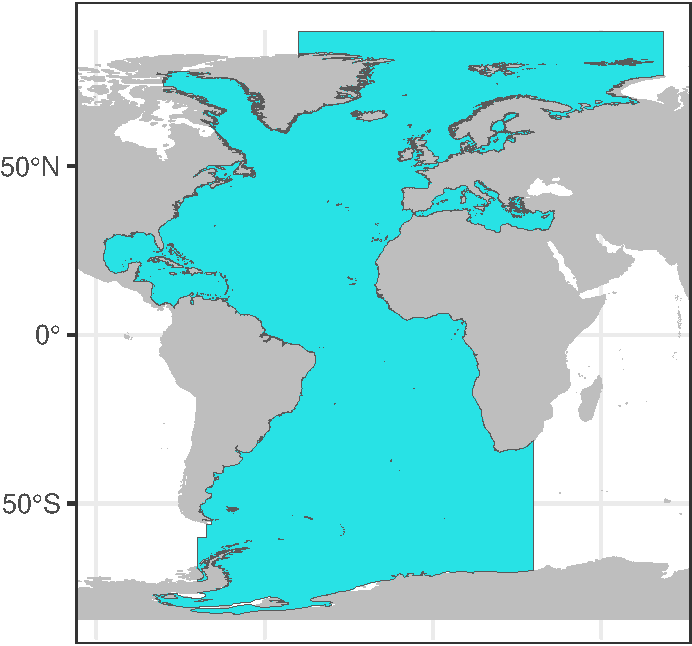
\includegraphics{_main_files/figure-latex/unnamed-chunk-18-1.pdf}

We save a base plot (p0) with the world map and our area of study in blue.

\begin{Shaded}
\begin{Highlighting}[]
\CommentTok{\# Basic ggplot}
\NormalTok{global }\OtherTok{\textless{}{-}} \FunctionTok{map\_data}\NormalTok{(}\StringTok{"worldHires"}\NormalTok{)}

\NormalTok{p0 }\OtherTok{\textless{}{-}} \FunctionTok{ggplot}\NormalTok{() }\SpecialCharTok{+} \FunctionTok{annotation\_map}\NormalTok{(}\AttributeTok{map =}\NormalTok{ global,}
    \AttributeTok{fill =} \StringTok{"grey"}\NormalTok{) }\SpecialCharTok{+} \FunctionTok{geom\_sf}\NormalTok{(}\AttributeTok{data =}\NormalTok{ study\_area.sf,}
    \AttributeTok{fill =} \DecValTok{5}\NormalTok{)}

\FunctionTok{print}\NormalTok{(p0)}
\end{Highlighting}
\end{Shaded}

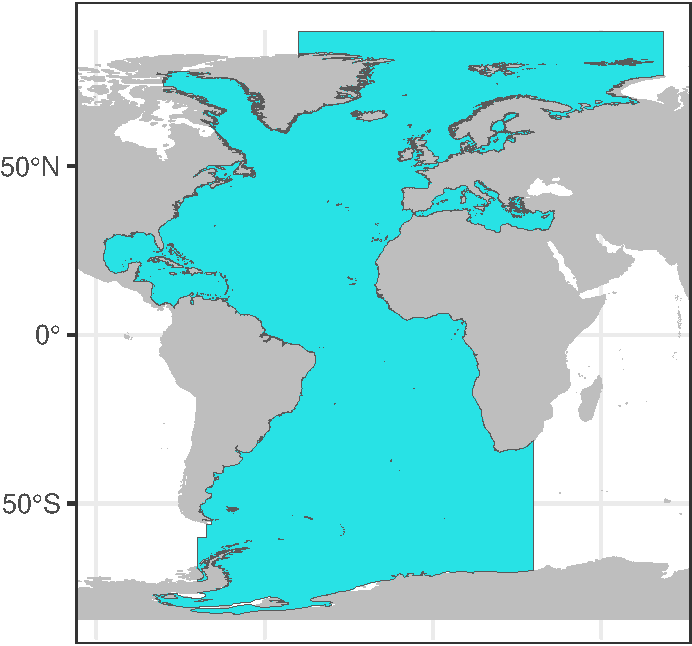
\includegraphics{_main_files/figure-latex/unnamed-chunk-19-1.pdf}

In order to generate a buffer around each occurrence data point, we need to work with euclidean distances, so first, we need to transform the decimal latitude and longitude values to UTM.

\begin{Shaded}
\begin{Highlighting}[]
\CommentTok{\# Function to find your UTM.}
\NormalTok{lonlat2UTM }\OtherTok{=} \ControlFlowTok{function}\NormalTok{(lonlat) \{}
\NormalTok{    utm }\OtherTok{=}\NormalTok{ (}\FunctionTok{floor}\NormalTok{((lonlat[}\DecValTok{1}\NormalTok{] }\SpecialCharTok{+} \DecValTok{180}\NormalTok{)}\SpecialCharTok{/}\DecValTok{6}\NormalTok{)}\SpecialCharTok{\%\%}\DecValTok{60}\NormalTok{) }\SpecialCharTok{+}
        \DecValTok{1}
    \ControlFlowTok{if}\NormalTok{ (lonlat[}\DecValTok{2}\NormalTok{] }\SpecialCharTok{\textgreater{}} \DecValTok{0}\NormalTok{) \{}
\NormalTok{        utm }\SpecialCharTok{+} \DecValTok{32600}
\NormalTok{    \} }\ControlFlowTok{else}\NormalTok{ \{}
\NormalTok{        utm }\SpecialCharTok{+} \DecValTok{32700}
\NormalTok{    \}}
\NormalTok{\}}

\NormalTok{(EPSG\_2\_UTM }\OtherTok{\textless{}{-}} \FunctionTok{lonlat2UTM}\NormalTok{(}\FunctionTok{c}\NormalTok{(}\FunctionTok{mean}\NormalTok{(df}\SpecialCharTok{$}\NormalTok{LON),}
    \FunctionTok{mean}\NormalTok{(df}\SpecialCharTok{$}\NormalTok{LAT))))}
\end{Highlighting}
\end{Shaded}

\begin{verbatim}
## [1] 32623
\end{verbatim}

\begin{Shaded}
\begin{Highlighting}[]
\CommentTok{\# Transform study\_area and data points}
\CommentTok{\# to UTMs (in m)}
\NormalTok{aux }\OtherTok{\textless{}{-}} \FunctionTok{st\_transform}\NormalTok{(study\_area.sf, EPSG\_2\_UTM)}
\NormalTok{df.sf.utm }\OtherTok{\textless{}{-}} \FunctionTok{st\_transform}\NormalTok{(df.sf, EPSG\_2\_UTM)}
\end{Highlighting}
\end{Shaded}

Now, we can create buffers of 100 km around the points and join the resulting polygons. Then this buffer is intersected with the area of study defining the area where the pseudo-absences can be generated. To visualize the defined areas, we plot the buffers in red and the area that we will use to generate pseudo-absences in green.

\begin{Shaded}
\begin{Highlighting}[]
\CommentTok{\# Create buffers of 100000m}
\NormalTok{buffer }\OtherTok{\textless{}{-}} \FunctionTok{st\_buffer}\NormalTok{(df.sf.utm, }\AttributeTok{dist =} \FloatTok{1e+05}\NormalTok{)}
\NormalTok{buffer }\OtherTok{\textless{}{-}} \FunctionTok{st\_union}\NormalTok{(buffer)}

\CommentTok{\# Intersect the are with the buffer}
\NormalTok{aux0 }\OtherTok{\textless{}{-}} \FunctionTok{st\_difference}\NormalTok{(aux, buffer)}

\CommentTok{\# ggplot for all data}
\NormalTok{p0 }\SpecialCharTok{+} \FunctionTok{geom\_sf}\NormalTok{(}\AttributeTok{data =}\NormalTok{ aux0, }\AttributeTok{fill =} \DecValTok{3}\NormalTok{) }\SpecialCharTok{+} \FunctionTok{geom\_sf}\NormalTok{(}\AttributeTok{data =}\NormalTok{ buffer,}
    \AttributeTok{fill =} \DecValTok{2}\NormalTok{)}
\end{Highlighting}
\end{Shaded}

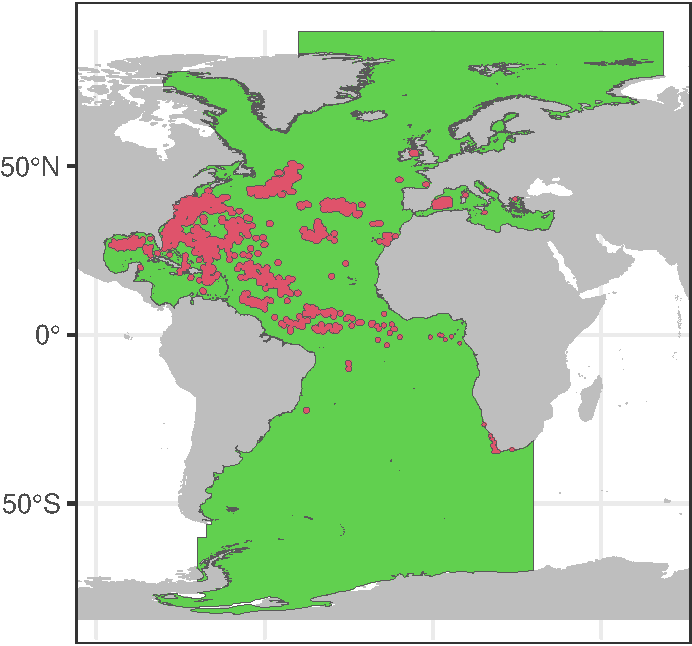
\includegraphics{_main_files/figure-latex/unnamed-chunk-21-1.pdf}

\begin{Shaded}
\begin{Highlighting}[]
\CommentTok{\# zoom}
\NormalTok{p0 }\SpecialCharTok{+} \FunctionTok{geom\_sf}\NormalTok{(}\AttributeTok{data =}\NormalTok{ aux0, }\AttributeTok{fill =} \DecValTok{3}\NormalTok{) }\SpecialCharTok{+} \FunctionTok{geom\_sf}\NormalTok{(}\AttributeTok{data =}\NormalTok{ buffer,}
    \AttributeTok{fill =} \DecValTok{2}\NormalTok{) }\SpecialCharTok{+} \FunctionTok{coord\_sf}\NormalTok{(}\AttributeTok{xlim =} \FunctionTok{c}\NormalTok{(}\SpecialCharTok{{-}}\DecValTok{95}\NormalTok{, }\SpecialCharTok{{-}}\DecValTok{82}\NormalTok{),}
    \AttributeTok{ylim =} \FunctionTok{c}\NormalTok{(}\DecValTok{22}\NormalTok{, }\DecValTok{31}\NormalTok{))}
\end{Highlighting}
\end{Shaded}

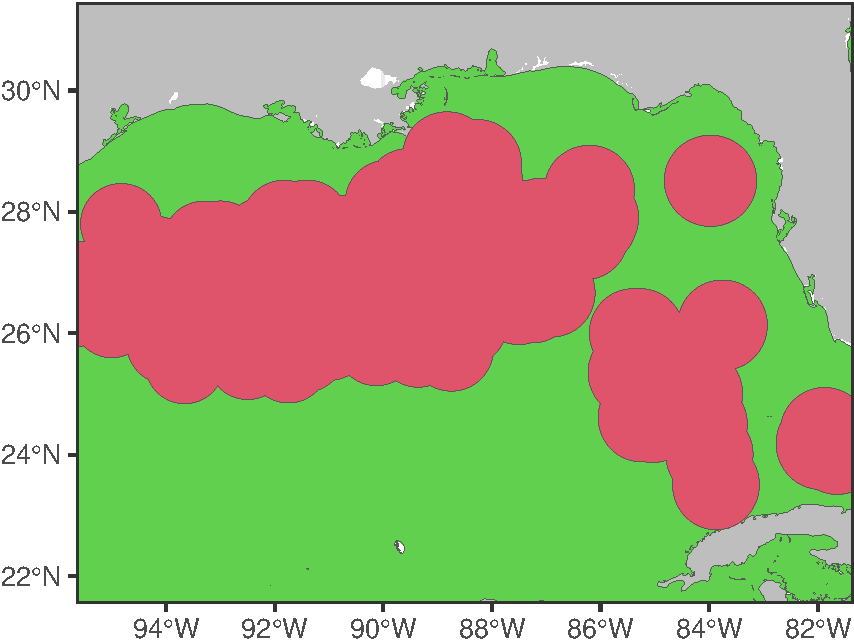
\includegraphics{_main_files/figure-latex/unnamed-chunk-21-2.pdf}

We create a data frame for pseudo-absences with the same dimensions as the presences data frame.

\begin{Shaded}
\begin{Highlighting}[]
\CommentTok{\# Generate the pseudo{-}absence data}
\CommentTok{\# frame}
\NormalTok{pseudo }\OtherTok{\textless{}{-}} \FunctionTok{matrix}\NormalTok{(}\AttributeTok{data =} \ConstantTok{NA}\NormalTok{, }\AttributeTok{nrow =} \FunctionTok{dim}\NormalTok{(df0)[}\DecValTok{1}\NormalTok{],}
    \AttributeTok{ncol =} \FunctionTok{dim}\NormalTok{(df0)[}\DecValTok{2}\NormalTok{])}
\NormalTok{pseudo }\OtherTok{\textless{}{-}} \FunctionTok{data.frame}\NormalTok{(pseudo)}
\FunctionTok{names}\NormalTok{(pseudo) }\OtherTok{\textless{}{-}} \FunctionTok{names}\NormalTok{(df0)}
\end{Highlighting}
\end{Shaded}

To generate the pseudo-absence data points, we sample randomly from the defined area and we extract their latitude and longitude to incorporate them in the created data frame. We set the occurrenceStatus equal to 0 as they are absences.

\begin{Shaded}
\begin{Highlighting}[]
\CommentTok{\# Set the seed}
\FunctionTok{set.seed}\NormalTok{(}\DecValTok{1}\NormalTok{)}

\CommentTok{\# Sample from the defined area}
\NormalTok{rp.sf }\OtherTok{\textless{}{-}} \FunctionTok{st\_sample}\NormalTok{(aux0, }\AttributeTok{size =} \FunctionTok{dim}\NormalTok{(df.sf.utm)[}\DecValTok{1}\NormalTok{],}
    \AttributeTok{type =} \StringTok{"random"}\NormalTok{)  }\CommentTok{\# randomly sample points}

\CommentTok{\# Transform to lat and lon and extract}
\CommentTok{\# coordinates as data.frame}
\NormalTok{rp.sf }\OtherTok{\textless{}{-}} \FunctionTok{st\_transform}\NormalTok{(rp.sf, }\DecValTok{4326}\NormalTok{)}
\NormalTok{rp }\OtherTok{\textless{}{-}} \FunctionTok{as.data.frame}\NormalTok{(}\FunctionTok{st\_coordinates}\NormalTok{(rp.sf))}
\NormalTok{pseudo}\SpecialCharTok{$}\NormalTok{LON }\OtherTok{\textless{}{-}}\NormalTok{ rp}\SpecialCharTok{$}\NormalTok{X}
\NormalTok{pseudo}\SpecialCharTok{$}\NormalTok{LAT }\OtherTok{\textless{}{-}}\NormalTok{ rp}\SpecialCharTok{$}\NormalTok{Y}

\CommentTok{\# Complete the rest of columns}
\NormalTok{pseudo}\SpecialCharTok{$}\NormalTok{scientificName }\OtherTok{\textless{}{-}}\NormalTok{ df0}\SpecialCharTok{$}\NormalTok{scientificName}
\NormalTok{pseudo}\SpecialCharTok{$}\NormalTok{occurrenceStatus }\OtherTok{\textless{}{-}} \DecValTok{0}
\end{Highlighting}
\end{Shaded}

We can plot the generated pseudo-absence data (in pink) in the map, together with the presence data points (in black).

\begin{Shaded}
\begin{Highlighting}[]
\NormalTok{p0 }\SpecialCharTok{+} \FunctionTok{geom\_sf}\NormalTok{(}\AttributeTok{data =}\NormalTok{ rp.sf, }\AttributeTok{col =} \DecValTok{6}\NormalTok{, }\AttributeTok{shape =} \DecValTok{4}\NormalTok{,}
    \AttributeTok{size =} \FloatTok{0.5}\NormalTok{) }\SpecialCharTok{+} \FunctionTok{geom\_sf}\NormalTok{(}\AttributeTok{data =}\NormalTok{ df.sf.utm,}
    \AttributeTok{col =} \DecValTok{1}\NormalTok{, }\AttributeTok{alpha =} \FloatTok{0.8}\NormalTok{, }\AttributeTok{size =} \FloatTok{0.5}\NormalTok{) }\SpecialCharTok{+} \FunctionTok{ggtitle}\NormalTok{(}\FunctionTok{unique}\NormalTok{(df}\SpecialCharTok{$}\NormalTok{scientificName))}
\end{Highlighting}
\end{Shaded}

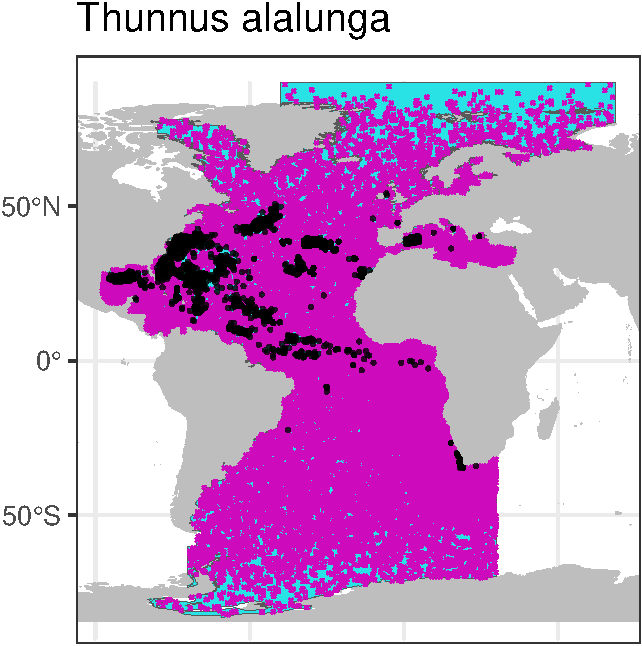
\includegraphics{_main_files/figure-latex/unnamed-chunk-24-1.pdf}

\begin{Shaded}
\begin{Highlighting}[]
\CommentTok{\# Zoom}
\NormalTok{p0 }\SpecialCharTok{+} \FunctionTok{geom\_sf}\NormalTok{(}\AttributeTok{data =}\NormalTok{ rp.sf, }\AttributeTok{col =} \DecValTok{6}\NormalTok{, }\AttributeTok{shape =} \DecValTok{4}\NormalTok{,}
    \AttributeTok{size =} \DecValTok{1}\NormalTok{) }\SpecialCharTok{+} \FunctionTok{geom\_sf}\NormalTok{(}\AttributeTok{data =}\NormalTok{ df.sf.utm,}
    \AttributeTok{col =} \DecValTok{1}\NormalTok{, }\AttributeTok{alpha =} \FloatTok{0.8}\NormalTok{, }\AttributeTok{size =} \FloatTok{0.5}\NormalTok{) }\SpecialCharTok{+} \FunctionTok{coord\_sf}\NormalTok{(}\AttributeTok{xlim =} \FunctionTok{c}\NormalTok{(}\SpecialCharTok{{-}}\DecValTok{95}\NormalTok{,}
    \SpecialCharTok{{-}}\DecValTok{82}\NormalTok{), }\AttributeTok{ylim =} \FunctionTok{c}\NormalTok{(}\DecValTok{23}\NormalTok{, }\DecValTok{31}\NormalTok{)) }\SpecialCharTok{+} \FunctionTok{ggtitle}\NormalTok{(}\FunctionTok{unique}\NormalTok{(df}\SpecialCharTok{$}\NormalTok{scientificName))}
\end{Highlighting}
\end{Shaded}

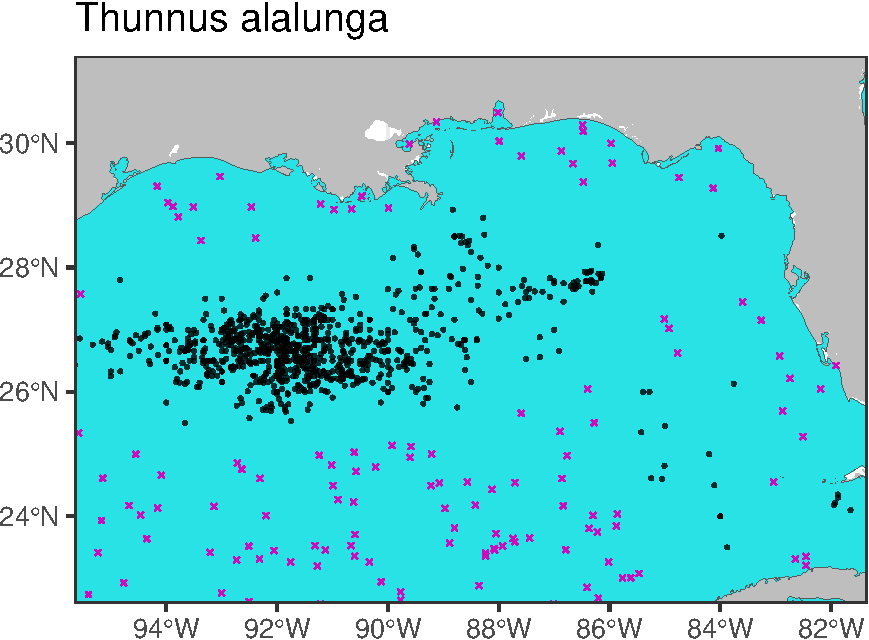
\includegraphics{_main_files/figure-latex/unnamed-chunk-24-2.pdf}

Finally we join the presence and pseudo-absence data frames selecting the columns of interest and save the new data frame.

\begin{Shaded}
\begin{Highlighting}[]
\CommentTok{\# Join the two data sets}
\NormalTok{PAdata }\OtherTok{\textless{}{-}} \FunctionTok{rbind}\NormalTok{(df0, pseudo)[, }\FunctionTok{c}\NormalTok{(}\StringTok{"scientificName"}\NormalTok{,}
    \StringTok{"LON"}\NormalTok{, }\StringTok{"LAT"}\NormalTok{, }\StringTok{"YEAR"}\NormalTok{, }\StringTok{"occurrenceStatus"}\NormalTok{)]}

\CommentTok{\# Save the final dataset of occurrence}
\CommentTok{\# and pseudo{-}absence points}
\FunctionTok{save}\NormalTok{(}\AttributeTok{list =} \FunctionTok{c}\NormalTok{(}\StringTok{"PAdata"}\NormalTok{), }\AttributeTok{file =} \FunctionTok{file.path}\NormalTok{(}\StringTok{"data"}\NormalTok{,}
    \StringTok{"outputs\_for\_modelling"}\NormalTok{, }\AttributeTok{file =} \StringTok{"PAdata.RData"}\NormalTok{))}
\end{Highlighting}
\end{Shaded}

\chapter{Acknowledgements}\label{acknowledgements}

This tutorial has been supported by the European Union's Horizon 2020 research and innovation programme under grant agreements No 862428 \href{https://missionatlantic.eu/}{MISSION ATLANTIC project}.

  \bibliography{references.bib}

\end{document}
